\documentclass{article}
\usepackage[landscape]{geometry}
\usepackage{url}
\usepackage{multicol}
\usepackage{amsmath}
\usepackage{esint}
\usepackage{amsfonts}
\usepackage{tikz}
\usetikzlibrary{decorations.pathmorphing}
\usepackage{amsmath,amssymb}
\usepackage{graphicx}
\usepackage{float}

\usepackage{colortbl}
\usepackage{xcolor}
\usepackage{mathtools}
\usepackage{amsmath,amssymb}
\usepackage{enumitem}
\makeatletter

\newcommand*\bigcdot{\mathpalette\bigcdot@{.5}}
\newcommand*\bigcdot@[2]{\mathbin{\vcenter{\hbox{\scalebox{#2}{$\m@th#1\bullet$}}}}}
\makeatother

\title{Unit 1 Summary Sheet}
\usepackage[T1]{fontenc}
\usepackage[utf8]{inputenc}
\usepackage[english]{babel}

\advance\topmargin-.8in
\advance\textheight3in
\advance\textwidth3in
\advance\oddsidemargin-1.5in
\advance\evensidemargin-1.5in
\parindent0pt
\parskip2pt
\newcommand{\hr}{\centerline{\rule{3.5in}{1pt}}}
%\colorbox[HTML]{e4e4e4}{\makebox[\textwidth-2\fboxsep][l]{texto}
\begin{document}

\begin{center}{\huge{\textbf{Unit 1 Summary Sheet}}}\\
\end{center}
\begin{multicols*}{3}

\tikzstyle{mybox} = [draw=black, fill=white, very thick,
    rectangle, rounded corners, inner sep=10pt, inner ysep=10pt]
\tikzstyle{fancytitle} =[fill=black, text=white, font=\bfseries]

%------------ Atomic Theory ---------------
\begin{tikzpicture}
\node [mybox] (box){%
    \begin{minipage}{0.3\textwidth}
    \textbf{Greek philosopher Democritus (400 BC)}: matter could not be divided into smaller and smaller pieces forever. He named the smallest piece of matter ``atomos'', meaning ``not to be cut''.\\
    \textbf{John Dalton's Model (early 1800s)}: all elements are composed of atoms, which are indivisible and indestructible particles.\\
    \textbf{J. J. Thomson (1897)}: atoms contain tiny negatively charged subatomic particles or electrons, he proposed the plum pudding model of the atom.\\
    \textbf{Ernest Rutherford}: discovered that atoms are mostly empty space with a tiny, dense, positively-charged nucleus. He did this through the gold foil experiment by shooting a beam of alpha particles at a sheet of gold foil, some of the particles were deflected.
    \end{minipage}
};
%------------ Atomic Theory Header ---------------------
\node[fancytitle, right=10pt] at (box.north west) {Atomic Theory};
\end{tikzpicture}

%------------ Atomic Structure ---------------
\begin{tikzpicture}
\node [mybox] (box){%
    \begin{minipage}{0.3\textwidth}
    Atoms can be further divided into subatomic particles (protons $p^{+}$, neutrons $n^{0}$, and electrons $e^{-}$).\\
    $p^{+}$: located in the nucleus of an atom.\\
    $n^{0}$: located in the nucleus of an atom.\\
    $e^{-}$: located in the orbitals of an atom.\\
    The \textbf{atomic number} (Z) of an atom is the number of protons in the nucleus.
    The \textbf{mass number} (A) is the total number of protons and neutrons.\\
    \# of protons = \# of electrons = atomic number\\
    \# of neutrons = mass number - atomic number
    \end{minipage}
};
%------------ Atomic Structure Header ---------------------
\node[fancytitle, right=10pt] at (box.north west) {Atomic Structure};
\end{tikzpicture}

%------------ Bohr-Rutherford Diagrams ---------------
\begin{tikzpicture}
\node [mybox] (box){%
    \begin{minipage}{0.3\textwidth}
    Each shell contains a fixed number of electrons: 2 $e^{-}$, 8 $e^{-}$, 8 $e^{-}$, 18 $e^{-}$.\\
    1. Draw the protons ($p^{+}$) and neutrons ($n^{0}$) in a circle, this represents the nucleus.\\
    2. Draw the electrons ($e^{-}$) around in orbital shells.
    \begin{figure}[H]
	\centering
	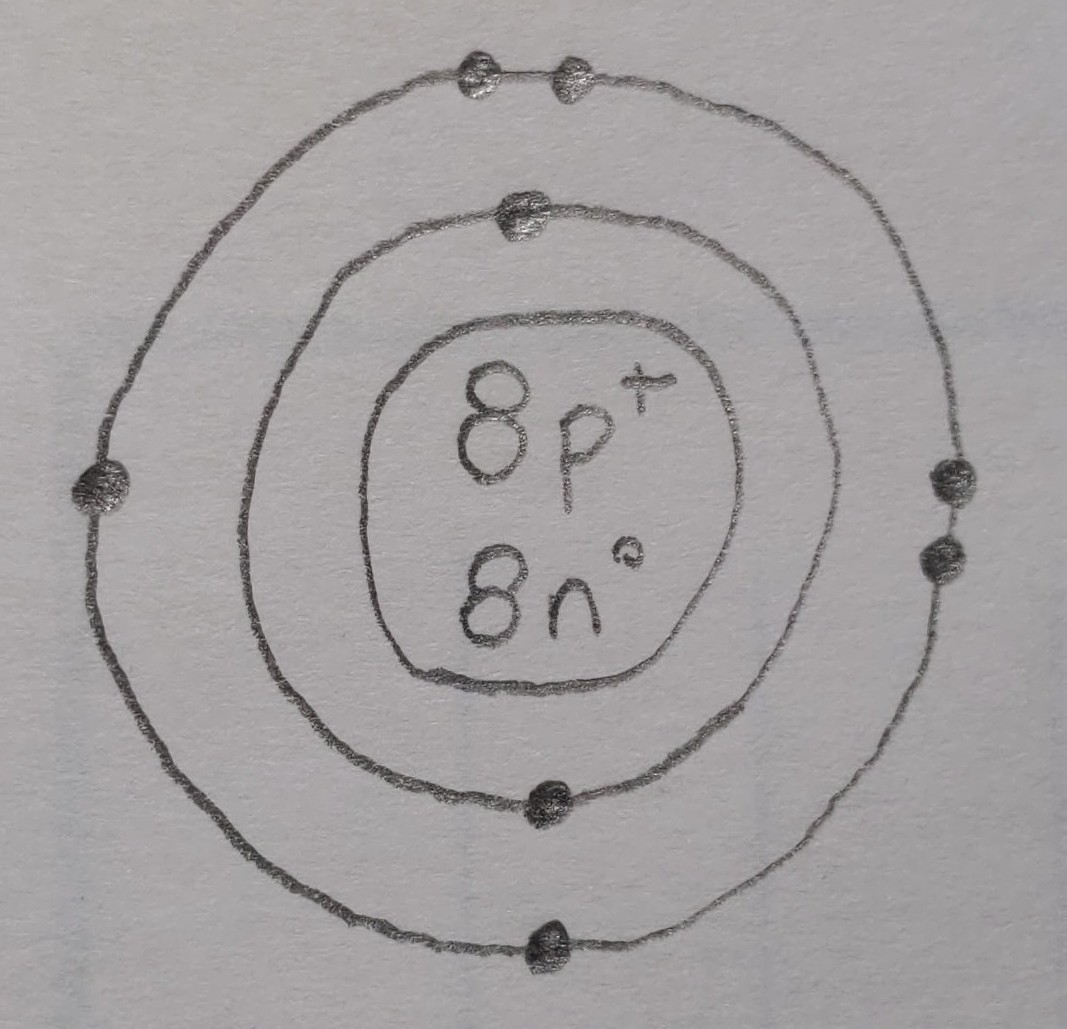
\includegraphics[scale=0.07]{diagrams/bohr.jpg}
	\caption{Oxygen Atom}
        \label{fig:bohr}
    \end{figure}
    \end{minipage}
};
%------------ Bohr-Rutherford Diagrams Header ---------------------
\node[fancytitle, right=10pt] at (box.north west) {Bohr-Rutherford Diagrams};
\end{tikzpicture}

%------------ Isotopes and Isotopic Abundance ---------------
\begin{tikzpicture}
\node [mybox] (box){%
    \begin{minipage}{0.3\textwidth}
    \textbf{Isotopes} are atoms of the same element that contain different number of neutrons but the same number of protons and electrons.\\
    The mass numbers of elements are not whole numbers due to isotopes. \\
    The \textbf{atomic mass} of an element is determined by calculating the weighted average of the masses of all isotopes of that element.\\
    \textbf{Isotopic abundance} refers to the percentage of an isotope in a sample of an element.\\
    Silicon has 3 isotopes found in nature: silicon-28, silicon-29, silicon-30.\\
    \textbf{Formula}: $avg.\,atomic\,mass=(\%\,abundance\times weight)+(\%\,abundance\times weight)...$
    \end{minipage}
};
%------------ Isotopes and Isotopic Abundance Header ---------------------
\node[fancytitle, right=10pt] at (box.north west) {Isotopes and Isotopic Abundance};
\end{tikzpicture}

%------------ Electron Configuration ---------------
\begin{tikzpicture}
\node [mybox] (box){%
    \begin{minipage}{0.3\textwidth}
    The electron ``clouds'' are orbitals. \\
    Schrödinger equation: $\hat{H}\psi=E\psi$ \\
    \textbf{s-orbitals} are spherically shaped, they have one orientation ($s^{2}$).\\
    \textbf{p-orbitals} are ``dumbbell'' shaped, they have three orientations ($p^{6}$).\\
    \textbf{d-orbitals} have five orientations ($d^{10}$).\\
    \textbf{f-orbitals} have seven orientations ($f^{14}$).\\
    \textbf{Aufbau Principle}: electrons occupy the orbitals of lowest energy first.\\
    \textbf{Pauli Exclusion Principle}: an atomic orbital can contain a maximum of only two electrons, and the two electrons must have opposite spins.\\
    \textbf{Hund's Rule}: electrons will first fill up each orbital before they start doubling up. \\ \\
    Unabbreviated and abbreviated configurations: \\
    iodine: $1s^{2}2s^{2}2p^{6}3s^{2}3p^{6}4s^{2}3d^{10}4p^{6}5s^{2}4d^{10}5p^{5}$ \\
    iodine: $[Kr]\,5s^{2}4d^{10}5p^{5}$
    \end{minipage}
};
%------------ Electron Configuration Header ---------------------
\node[fancytitle, right=10pt] at (box.north west) {Electron Configuration};
\end{tikzpicture}

%------------ Periodic Law and Trends ---------------
\begin{tikzpicture}
\node [mybox] (box){%
    \begin{minipage}{0.3\textwidth}
    \textbf{Dmitri Mendeleev} discovered the Periodic Law in 1869, he arranged the elements in order of increasing atomic mass.\\
    \textbf{Modern Periodic Law}: when elements are arranged in order of increasing atomic number, elements with similar properties recur at regular intervals.
    \end{minipage}
};
%------------ Periodic Law and Trends Header ---------------------
\node[fancytitle, right=10pt] at (box.north west) {Periodic Law and Trends};
\end{tikzpicture}

%------------ Atomic Radius ---------------
\begin{tikzpicture}
\node [mybox] (box){%
    \begin{minipage}{0.3\textwidth}
    Atomic radius \textbf{increases} as you move \textbf{down} a group: there are more energy levels $\rightarrow$ valence $e^{-}$ are further away from the nucleus.\\
    Atomic radius \textbf{decreases} as you move \textbf{left to right} across a period: there are more protons $\rightarrow$ valence $e^{-}$ are pulled more towards the nucleus.
    \end{minipage}
};
%------------ Atomic Radius Header ---------------------
\node[fancytitle, right=10pt] at (box.north west) {Atomic Radius};
\end{tikzpicture}

%------------ Ionic Radius ---------------
\begin{tikzpicture}
\node [mybox] (box){%
    \begin{minipage}{0.3\textwidth}
    The pattern is similar to the atomic radius, however, non-metals tend to be \textbf{larger} than metal ions from the same period.\\
    \textbf{Non-metals}: have added valence $e^{-}$ which increases repulsion $\rightarrow$ valence $e^{-}$ spread further apart.\\
    \textbf{Metals}: fewer valence $e^{-}$ $\rightarrow$ stronger nuclear pull causing them to be closer to the nucleus.
    \end{minipage}
};
%------------ Ionic Radius Header ---------------------
\node[fancytitle, right=10pt] at (box.north west) {Ionic Radius};
\end{tikzpicture}

%------------ Ionization Energy ---------------
\begin{tikzpicture}
\node [mybox] (box){%
    \begin{minipage}{0.3\textwidth}
    Ionization energy \textbf{decreases} as you move \textbf{down} a group: valence $e^{-}$ are further away from the nucleus $\rightarrow$ weaker pull from the $p^{+}$ which requires less energy to remove.\\
    Ionization energy \textbf{increases} as you move \textbf{left to right} across a period: more $p^{+}$ in the nucleus $\rightarrow$ valence $e^{-}$ are pulled more towards the nucleus which requires more energy to remove.
    \end{minipage}
};
%------------ Ionization Energy Header ---------------------
\node[fancytitle, right=10pt] at (box.north west) {Ionization Energy};
\end{tikzpicture}

%------------ Electronegativity ---------------
\begin{tikzpicture}
\node [mybox] (box){%
    \begin{minipage}{0.3\textwidth}
    A measure of an atom's ability to attract shared electrons to itself.\\
    Electronegativity \textbf{increases} as you move \textbf{left to right} across a period: more $p^{+}$ in the nucleus $\rightarrow$ stronger attraction for $e^{-}$. \\
    Electronegativity \textbf{increases} as you move \textbf{up} a group: less valence shells $\rightarrow$ stronger attraction for $e^{-}$.
    \begin{itemize}
        \item 0 - 0.4 = Non-to slightly polar covalent
	\item 0.5 < $\Delta EN$ < 1.7 = Polar covalent
	\item $\geq$ 1.7 = Ionic
    \end{itemize}
    \textbf{Polar molecules} have a dipole with oppositely charged ends with polar bonds inside the molecule. \\
    \textbf{Non-polar molecules} do not have charged ends.
    \end{minipage}
};
%------------ Electronegativity Header ---------------------
\node[fancytitle, right=10pt] at (box.north west) {Electronegativity};
\end{tikzpicture}

%------------ Lewis Structures ---------------
\begin{tikzpicture}
\node [mybox] (box){%
    \begin{minipage}{0.3\textwidth}
    \textbf{Gilbert Lewis} created this before the development of quantum mechanics.\\
    Noble gas configuration is the most \textbf{stable} due to its octet formation.\\
    Each bond contains \textbf{two electrons}.\\
    A metal and a non-metal achieve this by exchanging $e^{-}$'s = \textbf{ionic bond}\\
    A non-metal and a non-metal acheive this by sharing $e^{-}$'s = \textbf{covalent bond} \\ \\
    \small{
    \begin{tabular}{lp{3cm} l}
        & Have: & Want: \\
	& C 4$e^{-}$ $\times$ 1 = 4$e^{-}$ & 8$e^{-}$ \\
	+ & Br 7$e^{-}$ $\times$ 4 = 28$e^{-}$ & 32$e^{-}$ \\ \hline
	& Total: 32$e^{-}$ & 40$e^{-}$ \\
    \end{tabular}} \\ \\
    $40e^{-}-32e^{-}=8e^{-}$ \\
    $8e^{-}\div2e^{-}$ = 4 bonds
    \begin{figure}[H]
	\centering
	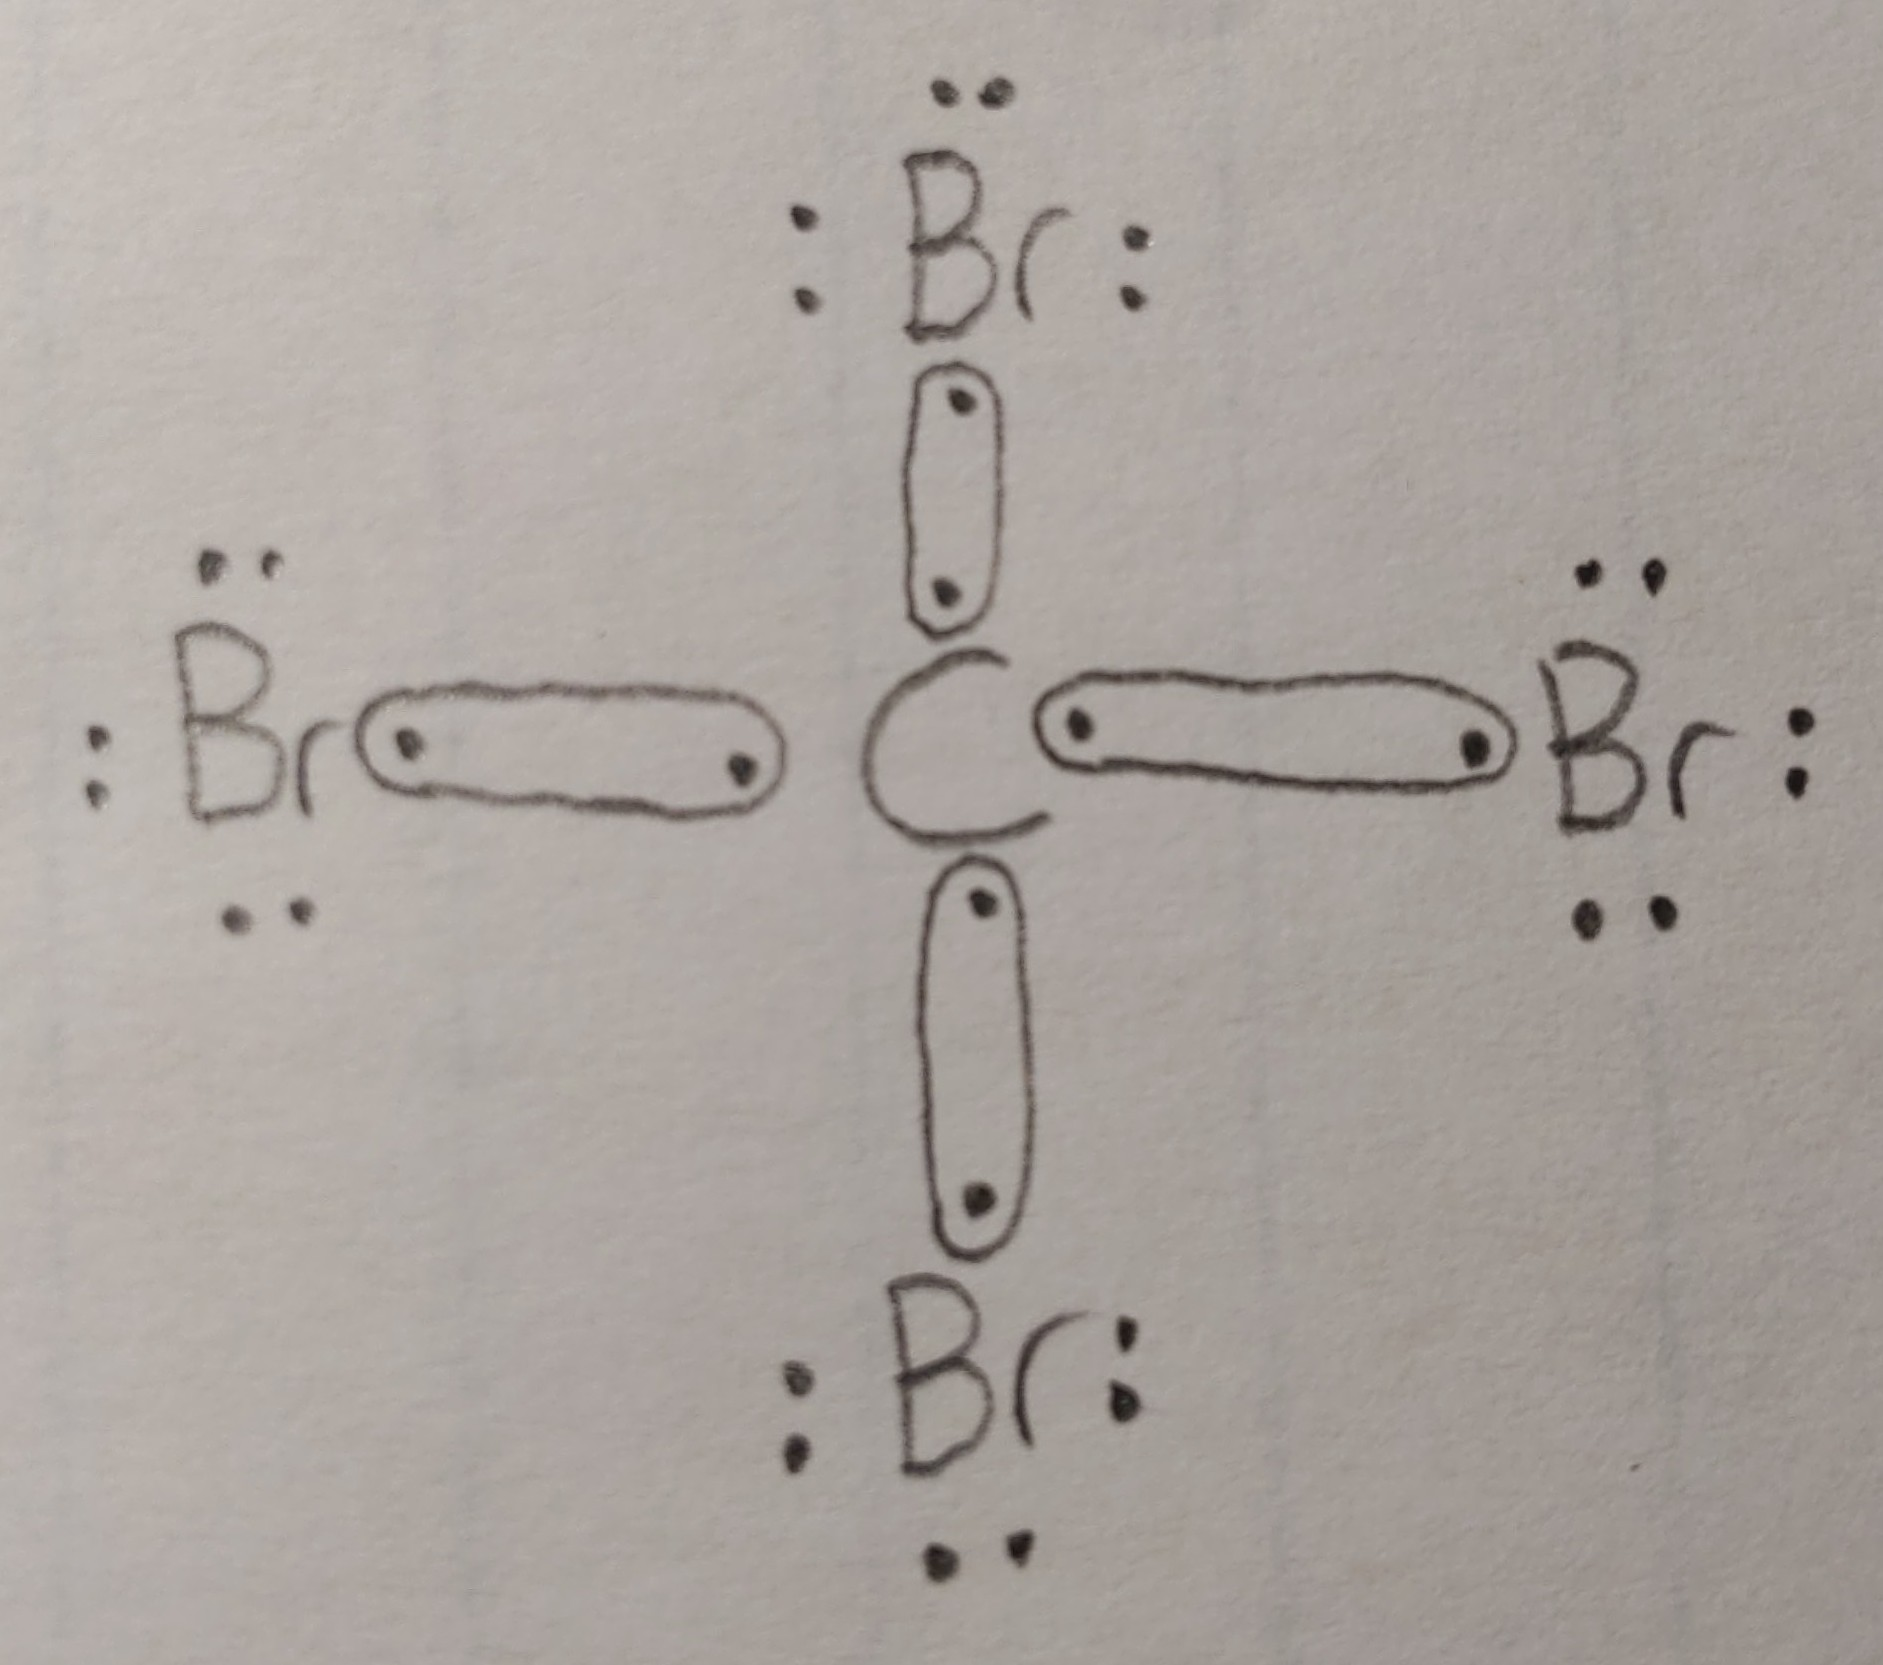
\includegraphics[scale=0.065]{diagrams/share.jpg}
        \caption{Carbon Tetrabromide}
        \label{fig:structure}
    \end{figure}
    \end{minipage}
};
%------------ Lewis Structures Header ---------------------
\node[fancytitle, right=10pt] at (box.north west) {Lewis Structures};
\end{tikzpicture}

%------------ Intermolecular Forces ---------------
\begin{tikzpicture}
\node [mybox] (box){%
    \begin{minipage}{0.3\textwidth}
    \textbf{covalent bond}: force which holds together the atoms in a molecule $\rightarrow$ very strong.\\
    \textbf{intermolecular forces}: attractive force between molecules $\rightarrow$ much weaker.\\
    \textbf{intramolecular forces}: attractive force between atoms $\rightarrow$ much stronger.\\
    \textbf{ionic compounds} $\rightarrow$ no intermolecular forces.\\
    Types of intermolecular forces (increasing strength):
    \begin{enumerate}
        \item \textbf{London dispersion}: occurs in all polar and non-polar molecules and unbonded atoms.
	\item \textbf{dipole-dipole}: electrostatic attraction between polar molecules.
	\item \textbf{hydrogen bonding}: stronger than regular dipole-dipole force, each molecule must have H covalently bonded to N, O, or F (large $\Delta EN$).
    \end{enumerate}
    \end{minipage}
};
%------------ Intermolecular Forces Header ---------------------
\node[fancytitle, right=10pt] at (box.north west) {Intermolecular Forces};
\end{tikzpicture}

%------------ Nomenclature ---------------
\begin{tikzpicture}
\node [mybox] (box){%
    \begin{minipage}{0.3\textwidth}
    \textbf{Binary Ionic Compounds}: metal and non-metal bonded together.\\
    e.g. magnesium chloride ($MgCl_{2}$)
    \begin{itemize}
        \item name of metal (cation) stays the same.
	\item add -ide to the root of the non-metal (anion).
    \end{itemize}
    \textbf{Multivalent Ions}: elements that have more than one possible valence.\\
    e.g. iron can be $Fe^{2+}$ or $Fe^{3+}$
    \begin{enumerate}
        \item Old system: use -ic for highest of 2 possibilities or -ous for lowest of 2 possibilities.
	\item Stock system (IUPAC): use Roman numerals to denote the charge.
    \end{enumerate}
    \textbf{Molecular Compounds}: non-metal and non-metal bonded together via covalent bonding.\\
    e.g. dinitrogen pentoxide ($N_{2}O_{5}$)
    \begin{enumerate}
        \item Add prefix to first word (omit ``mono'').
	\item Add prefix to second word and add -ide to root.
    \end{enumerate}
    \textbf{Polyatomic Ions}: ions which consist of two or more atoms. \\ \\
    \small{
    	\begin{tabular}{ | c c | c c | }
        \hline
	Nitrate & ${NO_{3}}^{1-}$ & Hydroxide & $OH^{1-}$ \\ \hline
	Chlorate & ${ClO_{3}}^{1-}$ & Ammonium & ${NH_{4}}^{1+}$ \\ \hline
	Carbonate & ${CO_{3}}^{2-}$ & Acetate & ${CH_{3}COO}^{1-}$ \\ \hline
	Sulfate & ${SO_{4}}^{2-}$ & Cyanide & ${CN}^{1-}$ \\ \hline
	Phosphate & ${PO_{4}}^{3-}$ & Permanganate & ${MnO_{4}}^{1-}$ \\
	\hline
	\end{tabular}} \\ \\ \\
    \textbf{Polyatomic Derivatives}: other polyatomic ions can be derived from the basic radicals. \\
    e.g. ${SO_{4}}^{2-}$ (Sulfate) $\rightarrow$ ${SO_{5}}^{2-}$ (Persulfate) \\
    e.g. ${SO_{4}}^{2-}$ (Sulfate) $\rightarrow$ ${SO_{3}}^{2-}$ (Sulfite) \\
    e.g. ${SO_{4}}^{2-}$ (Sulfate) $\rightarrow$ ${SO_{2}}^{2-}$ (Hyposulfite)
    \begin{itemize}
        \item per- \_\_\_ -ate $\rightarrow$ one more oxygen
        \item -ate $\rightarrow$ base
        \item -ite $\rightarrow$ one less oxygen
        \item hypo- \_\_\_ -ite $\rightarrow$ two less oxygen
    \end{itemize}
    \textbf{Adding a hydrogen to the radical}: adding a hydrogen to a polyatomic changes its charge. \\
    e.g. carbonate (${CO_{3}}^{2-}$) $\rightarrow$ bicarbonate (${HCO_{3}}^{1-}$) \\
    \textbf{Peroxides}: a radical of the form ${O_{2}}^{2-}$. \\
    e.g. sodium peroxide ($Na_{2}O_{2}$)
    \end{minipage}
};
%------------ Nomenclature Header ---------------------
\node[fancytitle, right=10pt] at (box.north west) {Nomenclature};
\end{tikzpicture}

%------------ Nomenclature Continued ---------------
\begin{tikzpicture}
\node [mybox] (box){%
    \begin{minipage}{0.3\textwidth}
    \textbf{Binary Acids}: contains only two elements (hydrogen and some other element).\\
    e.g. hydrochloric acid $HCl$ (aq)
    \begin{itemize}
        \item use the prefix ``hydro-''.
	\item add the suffix ``-ic''.
    \end{itemize}
    \textbf{Oxyacids}: contains polytatomic ions with oxygen in them.\\
    e.g. $CH_{2}O_{4}$ (aq) percarbonic acid \\
    e.g. $CH_{3}COOH$ (aq) acetic acid
    \begin{itemize}
        \item use -ic for polyatomic ions ending in ``-ate''.
	\item use -ous for polyatomic ions ending in ``-ite''.
    \end{itemize}
    \textbf{Hydrates}: a compound that has absorbed water molcules from an environment. \\
    e.g. $CuSO_{4}\cdot5H_{2}O$ copper (II) sulfate pentahydrate \\
    e.g. $BeSO_{4}\cdot4H_{2}O$ beryllium sulfate tetrahydrate
    \begin{itemize}
        \item use prefix for hydrate.
    \end{itemize}
    \end{minipage}
};
%------------ Nomenclature Continued Header ---------------------
\node[fancytitle, right=10pt] at (box.north west) {Nomenclature Continued};
\end{tikzpicture}

%------------ Electron Affinity ---------------
\begin{tikzpicture}
\node [mybox] (box){%
    \begin{minipage}{0.3\textwidth}
    Electron affinity \textbf{decreases} as you move \textbf{down} a group: valence $e^{-}$ are further away from the nucleus $\rightarrow$ weaker pull from the $p^{+}$ which releases less energy when new $e^{-}$ acquired.
    Electron affinity \textbf{increases} as you move \textbf{left to right} across a period: smaller radius $\rightarrow$ strong attraction between nucleus and valence $e^{-}$ $\rightarrow$ more energy is released when new $e^{-}$ is acquired.
    Exceptions exist in noble gases and in group 2.
    \end{minipage}
};
%------------ Electron Affinity Header ---------------------
\node[fancytitle, right=10pt] at (box.north west) {Electron Affinity};
\end{tikzpicture}

%------------ Radioisotopes ---------------
\begin{tikzpicture}
\node [mybox] (box){%
    \begin{minipage}{0.3\textwidth}
    Radioisotopes occur when at least one \textbf{unstable isotope} breaks down and releases radiation.\\
    \textbf{Radioactivity} is the spontaneous emission of radiation from the nucleus of an atom.
    \begin{itemize}
        \item alpha particle ($\alpha$) - positively charged particle.
        \item beta particle ($\beta$) - positive or negative particle.
	\item gamma ray ($\gamma$) - does not consist of particles, energy (photons) that has no mass or charge.
    \end{itemize}
    Unstable isotopes decay to become \textbf{more stable}, forming a new atom of a different element.
    \end{minipage}
};
%------------ Radioisotopes Header ---------------------
\node[fancytitle, right=10pt] at (box.north west) {Radioisotopes};
\end{tikzpicture}

\end{multicols*}
\end{document}
